\chapter{Introducción}

Esta investigación tiene como objetivo transformar las instrucciones de algoritmos de grafos en una representación visual e interactiva a través de un videojuego. Esta representación se destina a estudiantes de informática, con lo que se puede evaluar si el uso de herramientas interactivas con feedback visual mejora tanto el aprendizaje como la motivación.

El trabajo implica presentar a estudiantes de ciencias de la computación (CS) un videojuego que exhiba grafos. En este juego, el usuario debe ejecutar las instrucciones de los algoritmos con la asistencia de elementos visuales y auditivos.

El objetivo de esta investigación de tesis es identificar posibles diferencias en los niveles de motivación y comprensión de los algoritmos entre los estudiantes. Esto se medirá mediante una prueba que evaluará su conocimiento de los algoritmos de grafos.

El público objetivo son estudiantes de primer año de ciencias de la computación, aunque también es aplicable a estudiantes de ingeniería con conocimientos de programación. El requisito principal es que no hayan estudiado grafos previamente.

\section{Motivación}

La adopción de tecnologías digitales ha agilizado el acceso al conocimiento, permitiendo que estudiantes previamente excluidos ahora puedan acceder a la educación. Sin embargo, la educación en línea presenta desafíos propios \cite{UN2023ImpactDigitalTechnologies}. En este contexto, es crucial buscar metodologías que aceleren el aprendizaje con tecnologías adaptables, escalables y eficientes.

Se postula popularmente que la capacidad de atención de forma prolongada ha disminuido en las nuevas generaciones. Hay estudios que contradicen estas afirmaciones \cite{The_Role_of_Attention_Learning_Digital_Age}, indicando que las habilidades cognitivas de los estudiantes han cambiado, pero no necesariamente empeorado. Existen términos como ``doomsters'' y ``boosters'' \cite{Selwyn2014LookingF}, para descibrir la polarización entre estas miradas con respecto a la tecnología.

En lo que sí existe consenso, es que la tecnología y su portabilidad ha incrementado la cantidad de distracciones a las que se exponen
los estudiantes \cite{Zimmerman2011HandbookOS, Wang2022ComprehensivelySummarizeDistractions}. Se le llama multitasking al acto de intentar realizar más de una tarea a la vez. Se ha demostrado que esta práctica disminuye la productividad y el aprendizaje, aunque las personas creen que pueden hacer más de una cosa a la vez \cite{Domoff2019AddictivePU}.  Con la popularización de los smartphones y las clases en línea, el multitasking -desde hacer labores del hogar hasta sacar el celular y revisar alguna aplicación- durante clases se ha incrementado \cite{Wang2022ComprehensivelySummarizeDistractions}.

Una forma de distracción reconocida en la literatura es la interferencia motivacional, propuesta y explicada por Fries y Dietz \cite{Fries2007LearningMotivationalInterference}. Esta señala que la motivación respecto a la clase disminuye debido a la presencia de tentaciones más atractivas para la atención, como los smartphones. En este contexto, donde los estudiantes se ven tentados a distraerse, es importante buscar formas de mantenerlos motivados y enfocados durante las clases.
Los videjuegos educativos destacan porque tienen potencial como una herramienta complementaria para la enseñanza, evaluación y entretemiento para los estudiantes. Entre sus beneficios se destaca la motivación. En \cite{Bisson1996FunInLEarningPedagogicalRole} se indica que para disfrutar una actividad, primero se debe permitir a la mente de un individuo percibir tal actividad como motivante. 

Yu hace una revisión sistemática de la literatura \cite{Yu2020TheEffectsOfEducationGames} sobre los efectos de los videojuegos educativos en el aprendizaje de los estudiantes y su motivación. En este estudio, relativo a la motivación, se señala que el uso de videojuegos educativos como complemento afecta positivamente la motivación e incluso los logros académicos, pero también señala que han habido estudios que contradicen esta afirmación, por lo que se requiere más investigación en el área.

En el estudio mencionado, se asevera que el diseño del videojuego afecta totalmente el resultado final. Por ejemplo, los juegos de acción o realidad aumentada tenían mejores resultados que un juego tradicional, y que las mecánicas, elementos visuales y narrativos tienen un efecto significativo en el resultado final.

Considerando estos antecedentes, de que un videojuego educativo puede enseñar, es escalable, repetible y flexible, es que se presenta una oportunidad para analizar la percepción de estudiantes de computación con respecto a un videojuego educativo que enseñe algoritmos relacionados a grafos.

En la mayoría de los estudios citados previamente se indica que falta tener certeza respecto de la percepción de los usuarios al jugar videojuegos educativos y que se requiere indagar más. Por lo mismo, resulta conveniente emplear una prueba estandarizada para probar distintos diseños de videojuegos, con distintas poblaciones objetivo, pero cuyo resultado sea medido con el mismo estándar. Por esta razón, se utilizó un formulario basado en el modelo MEEGA+ \cite{meegaplus} para medir la motivación de los estudiantes, y una prueba de conocimiento para medir el aprendizaje de los estudiantes.


% Hablar que existen formas más eficientes de aprendizaje
% Revisar si el feedback inmediato ofrece ventajas sobre el feedback a largo plazo. 


\section{Objetivo General}

% Indicar aquí que queremos medir aprendizaje y motivación
El objetivo principal de este trabajo es medir el aprendizaje y la motivación de los estudiantes de computación al utilizar un videojuego educativo para instruir en algoritmos vinculados a grafos, incorporando las características expuestas en este documento.

\section{Objetivos Específicos}

% Determinar falencias, recomendaciones de diseño para un futuro videojuego
% Factores a considerar, como fecha en que se hace el estudio, la naturaleza de la muestra
% Su disponibilidad, etc
\begin{itemize}

\item Concebir una aplicación interactiva que visualice grafos y permita seguir los pasos relacionados con algoritmos que operan en dichos grafos.

\item Llevar a cabo una evaluación estandarizada para medir la percepción de los estudiantes respecto al videojuego creado.

\item Idear, desarrollar e implementar mecánicas de juego y una arquitectura de programación transferibles a otros videojuegos que instruyan en materias relacionadas con la programación.


\end{itemize}



\section{Marco teórico}

% All statistical model needs an assumption or a set of assumption to work correctly. As mention
% before, IRT unidimensional dichotomous models need to hold three principal assumptions:
% (i) The monotonicity in the relationship between the latent trait and the probability to
% answer a specific category (i.e., the shape of the Item Characteristic Curve (ICC)), (ii)
% the unidimensionality, and (iii) the Local independence principle. The variation on these
% assumptions for unidimensional polytomous IRT models is related to the first assumption.
% In that case, the ICC is a set of curves where only one of them satisfies the assumption (i).
% When assumption (ii) does not hold, multidimensional dichotomous and polytomous IRT
% models (MIRT) are appropriate, which allows more than one latent trait dimension. All these
% details are explained in the next subsections.
\subsection{Metodología de trabajo para validar videojuegose educativos}

Petri y Gresse von Wangenheim en \cite{HowGamesComputingEducationEvaluated}, antes de crear el modelo MEEGA+ cuya publicación sucedió el 2018 \cite{meegaplus}, hacen una revisión de literatura de cómo son evaluados los videojuegos educativos relacionados con la computación a partir de una muestra de 3617 artículos. Clasifica los estudios como verdaderos estudios, quasi-experimentales, no experimentales y ad-hoc según la metodología empleada.

% f the
% study uses either multiple groups or multiple moments of measurement, yet no random assignment, the study is classified as
% quasi-experimental. If the study does not use multiple groups, but is conducted in a systematic way, such as case studies (Yin,
% 2009), the study is classified as non-experimental. Studies executed in an unsystematic manner, without an explicit definition
% of the study and the measurement beforehand, are classified as ad-hoc studies.

Aquellos estudios que tenían múltiples grupos con asignación aleatoria eran considerados experimentales. Si el estudio usa múltiples grupos o múltiples momentos de medida sin asignación aleatoria, es considerado cuasi-experimental. Si no se emplean múltiples grupos, pero se hace de una forma sistemática con estudios de casos, es no experimental. Estudios que no son llevados de forma sistemática, sin una definición explícita del estudio y la forma de medirlo de antemano, son clasificados como estudios ad-hoc.

En una reseña, Calderón y Ruiz \cite{CalderonRuizReviewSeriousGamesEvaluation}, los autores identifican que la mayoría de los videojuegos educativos son evaluados en términos de aprendizaje, usabilidad y experiencia de usuario. Además, indican que la mayoría de los estudios se realizaron de una forma ad-hoc, sin sistematización. Este trabajo asevera que la mayoría de los estudios realizados utilizan cuestionarios y entrevistas como métodos de validación de resultados. Por otra parte, se crea una categorización de características que indican calidad en un juego, que posteriormente son utilizadas por \cite{meegaplus} en su cuestionario. Ejemplos de items evaluados son: Diseño de juego, satisfacción del usuario, usabilidad, motivación, resultados del aprendizaje, entre otros.

En su reseña sobre videojuegos serios, Calderón y Ruiz \cite{CalderonRuizReviewSeriousGamesEvaluation} también tabulan los tipos de procedimientos utilizados para validar estos trabajos, identificando tres tipos: 1) simple; 2) pre/post y 3) pre/post/post. 1) En el primero, los autores llevan a cabo una sesión con un juego serio, después de jugarlo, se aplican los mecanismos de evaluación a los jugadores; 2) En el pre/post, la prueba tiene dos etapas de evaluación. Uno antes del juego serio, y otro después, de manera que se establece el conocimiento anterior a la prueba; 3) Para el caso pre/post/post se hace, además de las pruebas pre y post, una prueba posterior semanas después para analizar los niveles de retención. Respecto a las frencuencias, 50 de 89 de estos estudios se hicieron con una metodología simple y el 55\% lo hizo con tamaños muestrales inferiores a 40 \cite{CalderonRuizReviewSeriousGamesEvaluation}.

Apoyándose en esta conclusión, Petri y Christiane Gresse von Wangenheim, en su reseña de literatura sobre videojuegos educativos \cite{HowGamesComputingEducationEvaluated} aseveran que la mayoría de los estudios sobre videojuegos educativos son realizados de una manera ad-hoc en términos de diseño de investigación, medición, recolección de datos y análisis. Sin embargo, destacan el modelo MEEGA \cite{meegaplusQualityEvaluationPage}, indicando que ha sido utilizado además en otras áreas distintas de la computación, proporcionando mayor sistematización y logrando que los trabajos basados en este modelo tengan mayor validez científica.


\subsection{Teoría de respuesta al ítem, Item Response Theory o IRT, intuición cualitativa}

Es un modelo estadístico utilizado utilizado por muchos tests globales como pruebas de inglés como lengua extranjera y el programa para la evaluación de estudiantes internacional. La cualidad que se le destacad es que permite evaluar propiedades estadísticas de forma detallada sobre cada item (o pregunta según sea el caso), viendo la dificultad y la capacidad de diferenciación de cada pregunta \cite{Linden2015HandbookOI, IRTShojima2022}.

Los modelos basados en IRT se basan en tres asunciones: Primero, existe una relación funcional entre la rasgo latente que se busca medir y la probabilidad de responder un ítem (o pregunta) en una cierta categoría, por ejemplo, en desacuerdo, de acuerdo o ninguno \cite{CalderonStatisticalIRT}.

Un segundo supuesto es que existe una escala continua y unidimensional de habilidad denotada como $\theta$ (parámetro theta). Esta es una suposición fuerte, pues los datos nunca son compeletamente unidimensionales, sin embargo, existen técnicas para verificar la unidimensionalidad de los datos de testeo \cite{IRTShojima2022}. Si se quieren medir más características al mismo tiempo, existen otros modelos de IRT multidimensionales \cite{Reckase2009MultidimensionalIRT}.

El tercer supuesto es la independencia local, la persona responde de forma independiente a cada uno de los items o preguntas de la prueba, sin influenciar la respuesta de una pregunta la respuesta de otra \cite{CalderonStatisticalIRT}.

Por definición, $\theta$ está en el rango $]-\infty, \infty [$, pero prácticamente la totalidad de los datos se encuentra en el rango aproximado de $]-3, 3[$. Un valor $\theta = 0$ se asume como un nivel promedio \cite{IRTShojima2022}. 

Existen distintos modelos logísticos para evaluar $\theta$. El que se usa en este trabajo es el modelo logístico de 2 parámetros (2PLM o Two-Parameter Logistic Model) y otra variante de tres parámetros. Los parámetros en estos casos buscan representar rasgos asociados a cada ítem o pregunta. El de 2 parámetros incluye dificultad y discriminación, aunque en español se podría interpretar mejor como distinción o graduación, asociado a indicar la probabilidad entre elegir un valor u otro \cite{CalderonStatisticalIRT}.  El valor de $\theta$ se puede aproximar utilizando el método bayesiano EAP (Expected A Posteriori), el cual se calcula utilizando los paquetes de R \textit{mirt} \cite{RMIRT} y \textit{mirtCAT} \cite{RPackageMIRTCAT} aplicados en este trabajo. 

El modelo 2PLM se compone del parámetro dificultad $b_j$ y de discriminación $a_j$ asignados para cada pregunta. Este último representa la pendiente de la curva e indica en qué medida el ítem diferencia a los examinados con un nivel en el rasgo latente por encima o debajo del parámetro de dificultad \cite{TeoriaRespuestaAlItemPsicologia}. En un modelo con respuestas correctas e incorrectas, un ítem con un parámetro de dificultad mayor $b_j$ será respondido incorrectamente con mayor probabilidad para casi cualquier nivel de $\theta$ \cite{IRTShojima2022}.


\begin{figure}[h]
	\centering
	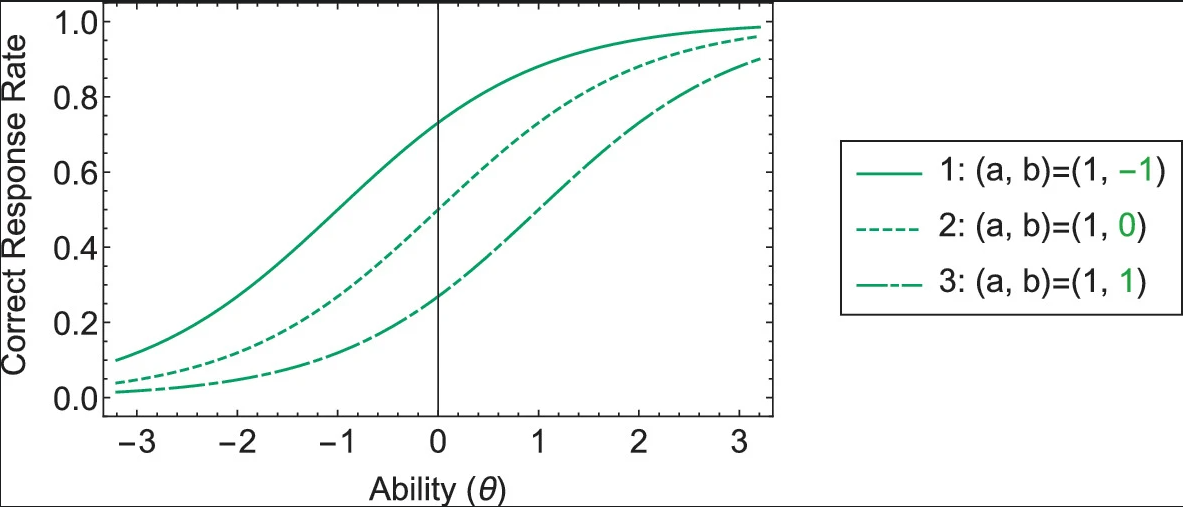
\includegraphics[scale=.5]{imagenes/IRTparambdifficulty.png}
	\caption{Probabilidad de responder correctamente para distintos valores del parámetro dificultad b}
	\label{ParamDifficulty}
\end{figure}


Es importante destacar que cada ítem discrimina mejor en torno a valores de $\theta$ que sean cercanos al parámetro de locación $b$. Además, un parámetro $a$ indica que el item es un mejor indicador para $\theta$, pero teniendo en consideración que este poder discriminativo funciona mejor cuando $\theta \approx b$. Por esta razón, cada pregunta por separado entrega información acerca del valor $\theta$ que se quiere obtener, de manera que las preguntas deben estar formuladas de tal manera que permitan distinguir distintos niveles del rasgo a evaluar \cite{TeoriaRespuestaAlItemPsicologia}.

Aplicando este modelo a una escala de Likert de formato ordinal, para cada pregunta se indican 4 parámetros b, para diferenciar entre los niveles 1) Muy en desacuerdo; 2) En desacuerdo; 3) Ni en desacuerdo ni de acuerdo; 4) De acuerdo y 5) Muy de acuerdo \cite{TeoriaRespuestaAlItemPsicologia, meegaplusQualityEvaluationPage}. De esta manera, a medida que $\theta$, la calidad de juego es mejor según \cite{meegaplusQualityEvaluationPage}, las respuestas más tenderán a ser del formato Muy de acuerdo, a excepción de algunas preguntas que no se incluyen en la valoración. El script de R utilizado para el cálculo de $\theta$ se encuentra disponible en \cite{meegaplusQualityEvaluationPage}.

Las fórmulas empleadas, demostraciones relacionadas con IRT o mostrar cómo afectan los distintos parámetros al resultado final está fuera del alcance de este estudio, principalmente porque los paquetes de R se encargan de realizar este trabajo.

\subsection{Motores de videojuegos: Godot}

Existen diversos motores de videojuegos, como Unreal Engine \cite{UE}, Unity \cite{Unity} y Godot \cite{Godot}. Este último resalta por ser completamente gratuito, de código abierto y poseer una comunidad que también participa activamente en el desarrollo del motor \cite{GodotGithubRepository}. La principal ventaja que ofrecen los motores de videojuegos es ofrecer un programa monolítico capaz de integrar diversas funcionalidades para distintos tipos de profesionales. Por ejemplo, ofrecen interfaces para integrar animaciones, así como trabajo con efectos visuales, de audio. Además, vienen con librerías integradas que se suelen utilizar en videojuegos, como colisiones, texturizado o composición de elementos, permitiendo unir la representación visual, auditiva y programática de un personaje. Los motores de videojuegos permiten exportar la aplicación a distintas plataformas sin necesidad de modificar el código \cite{GodotExport}.

Godot utiliza principalmente dos lenguajes de programación, GDScript, similar a Python, y C#. Para este trabajo se utilizaron ambos. El primero permite prototipar rápidamente debido a su simpleza e integración con el motor. El último es más rápido, pero hay características del motor que no están integradas en la versión utilizada durante este trabajo, que es la 3.5.2 \cite{GodotCSharpGDDifferences}.

